\documentclass[10pt,a4paper]{extarticle}
\usepackage[margin=2.1cm]{geometry}
\usepackage[T1]{fontenc}
\usepackage{newtxtext,newtxmath}
\usepackage{microtype,booktabs,graphicx,xcolor,enumitem,multirow,array,makecell}
\usepackage[font=small,labelfont=bf,skip=4pt]{caption}
\usepackage[most]{tcolorbox}
\usepackage[colorlinks,linkcolor=blue!50!black,citecolor=blue!50!black,urlcolor=blue!50!black]{hyperref}
\usepackage{float}
\setlist{nosep,leftmargin=1.3em,topsep=2pt}
\setlength{\parskip}{3pt}
\setlength{\parindent}{0pt}
\renewcommand{\arraystretch}{1.12}
\definecolor{good}{RGB}{0,110,60}
\definecolor{bad}{RGB}{170,30,30}
\newcommand{\pass}{\textcolor{good}{\textbf{PASS}}}
\newcommand{\fail}{\textcolor{bad}{\textbf{FAIL}}}
\newcommand{\yes}{\textcolor{good}{\textbf{yes}}}
\newcommand{\no}{\textcolor{bad}{\textbf{no}}}
\newcommand{\code}[1]{\texttt{\small #1}}
% sealed per-task
\newcommand{\SealedRows}{%
LOOP\_SEATTLE/5T/long & 0.558 & 0.591 & \textbf{0.534} & 1.044 & 0.944 \\
LOOP\_SEATTLE/5T/medium & 0.562 & 0.592 & \textbf{0.529} & 1.062 & 0.948 \\
LOOP\_SEATTLE/5T/short & 0.577 & 0.582 & \textbf{0.539} & 1.071 & 0.992 \\
LOOP\_SEATTLE/H/short & 0.612 & 0.616 & \textbf{0.572} & 1.071 & 0.993 \\
bitbrains\_fast\_storage/5T/long & 0.698 & 0.688 & \textbf{0.627} & 1.113 & 1.015 \\
bitbrains\_fast\_storage/5T/medium & 0.718 & 0.689 & \textbf{0.688} & 1.044 & 1.042 \\
bitbrains\_fast\_storage/5T/short & \textbf{0.484} & 0.486 & 0.520 & 0.930 & 0.995 \\
bitbrains\_fast\_storage/H/short & 0.768 & 0.786 & \textbf{0.758} & 1.014 & 0.977 \\
bitbrains\_rnd/5T/long & 0.765 & \textbf{0.700} & 0.752 & 1.018 & 1.094 \\
bitbrains\_rnd/5T/medium & 0.646 & 0.621 & \textbf{0.597} & 1.081 & 1.039 \\
bitbrains\_rnd/5T/short & 0.408 & 0.432 & \textbf{0.407} & 1.002 & 0.944 \\
bitbrains\_rnd/H/short & 0.525 & \textbf{0.513} & 0.557 & 0.944 & 1.023 \\
car\_parts\_with\_missing/short & 0.632 & 0.647 & \textbf{0.626} & 1.010 & 0.977 \\
electricity/15T/long & 0.854 & \textbf{0.798} & 0.903 & 0.946 & 1.071 \\
electricity/15T/medium & 0.606 & \textbf{0.532} & 0.539 & 1.125 & 1.139 \\
electricity/15T/short & \textbf{0.571} & 0.582 & 0.604 & 0.944 & 0.980 \\
electricity/D/short & \textbf{0.526} & 0.534 & 0.584 & 0.900 & 0.984 \\
electricity/H/long & \textbf{0.621} & 0.666 & 0.626 & 0.992 & 0.933 \\
electricity/H/medium & 0.656 & 0.681 & \textbf{0.607} & 1.081 & 0.964 \\
electricity/H/short & 0.765 & 0.749 & \textbf{0.673} & 1.137 & 1.021 \\
kdd\_cup\_2018\_with\_missing/H/short & \textbf{0.530} & 0.538 & 0.552 & 0.959 & 0.985 \\
m4\_daily/short & 0.918 & \textbf{0.903} & 0.903 & 1.017 & 1.017 \\
m4\_monthly/short & 0.713 & 0.690 & \textbf{0.647} & 1.103 & 1.034 \\
m4\_quarterly/short & 0.742 & 0.751 & \textbf{0.621} & 1.195 & 0.988 \\
m4\_yearly/short & 0.853 & 0.988 & \textbf{0.660} & 1.293 & 0.863 \\
solar/10T/short & 0.749 & \textbf{0.712} & 0.748 & 1.002 & 1.052 \\
solar/H/short & 0.762 & 0.764 & \textbf{0.744} & 1.024 & 0.998 \\
temperature\_rain\_with\_missing/short & \textbf{0.527} & 0.527 & 0.536 & 0.983 & 0.999 \\
}
\newcommand{\DatasetRows}{%
bizitobs\_service & 3 & 0.498 & 0.849 \\
bizitobs\_application & 3 & 0.518 & 0.958 \\
jena\_weather & 7 & 0.968 & 0.979 \\
hierarchical\_sales & 2 & 0.974 & 0.962 \\
saugeenday & 3 & 0.987 & 1.013 \\
bizitobs\_l2c & 6 & 0.988 & 0.892 \\
SZ\_TAXI & 4 & 0.990 & 1.000 \\
bitbrains\_rnd & 4 & 0.991 & 1.003 \\
us\_births & 3 & 0.994 & 1.050 \\
ett2 & 8 & 0.994 & 0.997 \\
restaurant & 1 & 0.999 & 0.984 \\
electricity & 8 & 1.003 & 0.996 \\
kdd\_cup\_2018\_with\_missing & 4 & 1.006 & 0.994 \\
ett1 & 8 & 1.012 & 1.011 \\
hospital & 1 & 1.013 & 0.996 \\
car\_parts\_with\_missing & 1 & 1.020 & 0.974 \\
m4\_monthly & 1 & 1.021 & 0.975 \\
solar & 8 & 1.030 & 0.999 \\
bitbrains\_fast\_storage & 4 & 1.037 & 1.019 \\
LOOP\_SEATTLE & 7 & 1.048 & 0.969 \\
m4\_weekly & 1 & 1.063 & 1.031 \\
temperature\_rain\_with\_missing & 1 & 1.092 & 1.120 \\
m4\_daily & 1 & 1.121 & 1.096 \\
m4\_quarterly & 1 & 1.126 & 1.002 \\
M\_DENSE & 4 & 1.178 & 0.988 \\
m4\_yearly & 1 & 1.197 & 0.935 \\
m4\_hourly & 1 & 1.213 & 1.076 \\
covid\_deaths & 1 & 1.358 & 1.056 \\
}


\title{\vspace{-1.2cm}\textbf{Alma: Compact JEPA Time-Series Foundation Models and World Models}\\[4pt]
\large End-to-End Progress Report --- Alma v1, v2, v3 and Alma-WM1/WM2,\\ with Sealed, Pre-Registered Validation against Telos-Small}
\author{Alma project\\ \small Report generated 18 November 2026 from the raw run artefacts}
\date{}

\begin{document}
\maketitle
\vspace{-0.6cm}

\begin{tcolorbox}[colback=gray!6,colframe=gray!50,boxrule=0.5pt,arc=1pt,left=6pt,right=6pt,top=4pt,bottom=4pt,title=\textbf{Abstract},fonttitle=\small,coltitle=black,colbacktitle=gray!20]
\small
We report the full development and validation of \emph{Alma}, a family of compact time-series foundation
forecasters (v1: 21.4M, v2: 27.9M, v3: 61.8M parameters) and action-conditioned JEPA world models
(Alma-WM1/WM2), all trained on a single 16\,GB Apple M4 laptop GPU. The reference competitor is
Telos-Small (50.1M parameters), a time-series JEPA. All headline numbers come from a pre-registered
validation protocol with sealed outputs, fresh hold-out windows, paired $t$-tests and Holm correction.

\textbf{Forecasting.} On the full GIFT-Eval benchmark (97 configurations), Alma v3 reaches
\textbf{39.57\% CRPS skill} and \textbf{21.93\% MASE skill} over Seasonal Naive, against 38.33\% and 19.10\% for
Telos-Small and 38.76\% / 20.91\% for Alma v2. On the 51 tasks scored on identical windows, v3's
geometric-mean CRPS is 5.3\% below Telos-Small's (ratio 0.947, $t=1.77$, not significant). However, on our
\emph{sealed}, pre-registered test (8{,}300 fresh windows, 28 tasks), Telos-Small is better:
v3/Telos CRPS ratio \textbf{1.036} (95\% CI [1.007, 1.068], $t=-2.35$, v3 wins 29\% of tasks), and v3 is
statistically tied with v2 (0.999). The leaderboard advantage is concentrated in two BizITObs datasets;
excluding their 6 tasks, v3 is 2.3\% behind Telos on GIFT-Eval as well. \textbf{Conclusion: Alma v3 is
competitive with Telos-Small but does not beat it under our pre-registered criterion.}

\textbf{World model.} Alma-WM2 (64.4M parameters) earns the claim tier
\emph{``leak-free and reproducible''} (wm1 earned none). It beats an ARX(24,24) baseline at every horizon
beyond 16 steps (0.87--0.93), on the held-out \emph{tanks} family (0.919), and in 6 of 8 simulated
families, but not at one-step prediction (1.048), not significantly on counterfactuals (0.981, $t=0.7$),
and not in model-predictive control (1.087). Calibration (76.9\% for an 80\% interval) and the OOD
detector (AUROC 0.53) fail their gates.

\textbf{Main lesson.} Scaling the model $2.2\times$ and training longer did not move the sealed result:
the development score improved for 10k steps and then degraded while training loss kept falling.
The binding constraint is training data diversity, not model capacity.
\end{tcolorbox}

\tableofcontents
\clearpage

%=====================================================================
\section{Objectives and scope}
The project goals, as set by the project owner, were:
\begin{enumerate}
\item Build a time-series foundation model that beats Telos-Small and can serve as a strong
foundation model.
\item Build a complete JEPA \emph{world model} that predicts how a system responds to actions, and validate it
with the project's validation engine (\code{WORLD\_MODEL\_VALIDATION\_ENGINE.md}): pre-registration, sealed hold-outs,
gates 0--14 and claim tiers.
\item For v3 specifically: (i) grow to 12$\times$512 ($\approx$60M parameters) warm-started from v2;
(ii) train longer with more weight on long horizons; (iii) add a stride-32 path so 8k contexts are affordable;
(iv) add a JEPA objective so the forecaster shares one JEPA backbone with the world model;
(v) evaluate on a fresh sealed set and on the full GIFT-Eval benchmark; (vi) run this after wm2's training and validation.
\end{enumerate}
All six v3 items were implemented and executed. This report states for every result whether it is a
\emph{sealed, pre-registered} result or a \emph{descriptive} one, and reports negative results in full.

%=====================================================================
\section{Reference model: Telos-Small}
Telos-Small is a 50.1M-parameter time-series JEPA: causal Welford normalisation followed by \code{asinh}, patches of
32, a 12-block two-stream transformer with variate attention, a 2-block JEPA predictor and a 21-quantile monotone head,
trained on GiftEvalPretrain plus synthetic data for 43{,}591 steps on 2$\times$P100. Its model card reports 43.21\% GIFT
CRPS skill. On our harness (9-quantile CRPS, $\le$1{,}000 windows per task) it scores \textbf{38.33\%}; that figure is the
reference throughout, and every model, including Telos, is run through the identical harness.

%=====================================================================
\section{Model lineage}
\begin{table}[H]
\centering\small
\caption{All models trained in this project. Parameters are counted from the saved checkpoints.}
\label{tab:lineage}
\setlength{\tabcolsep}{4pt}
\resizebox{\linewidth}{!}{\begin{tabular}{@{}llrlll@{}}
\toprule
Model & Type & Params & Init & Training & Key change \\
\midrule
Alma v1 & forecaster & 21.4M & scratch & 20k steps $\times$ 64 & causal patch decoder, per-token quantiles \\
Alma v2 & forecaster & 27.9M & v1 @20k & 10k $\times$ 32 (best @6k) & direct horizon 1{,}024, window 4{,}096 \\
Alma-WM1 & world model & 36.4M & v2 @6k & 8k $\times$ 32 & action-conditioned JEPA predictor \\
Alma-WM2 & world model & 64.4M (36.5M trained) & WM1 @8k & 28k $\times$ 32 & frozen v2 path, in-model ARX prior \\
Alma v3 & forecaster & 61.8M (+7.65M JEPA head) & v2 @6k (grown) & 20k $\times$ 32 (best @10k) & 12$\times$512, stride-32 path, JEPA, balanced loss \\
Telos-Small & reference & 50.1M & --- & 43{,}591 steps, 2$\times$P100 & --- \\
\bottomrule
\end{tabular}}
\end{table}

%=====================================================================
\section{Data}
\textbf{Real pretraining data.} Salesforce \emph{GiftEvalPretrain}, which by construction does not overlap the GIFT-Eval
test windows. We used \code{data-*.arrow} files only, one shard for large sources, thinned CMIP6/ERA5/LargeST, split
multivariate series into channels, and capped series at 16{,}384 points and sources at 60k series. Result:
\textbf{94 sources, 433{,}528 series, 1.20B points} (4.8\,GB packed).

\textbf{Mixture.} 55\% real windows (sources sampled $\propto\sqrt{\text{points}}$, 20\% temporally downsampled),
15\% TSMixup combinations, 30\% synthetic series (40\% KernelSynth-style Gaussian processes, 60\% structural:
trend, seasonality, AR noise, intermittency, level shifts, spikes, multiplicative effects); random missing blocks and
patch offsets.

\textbf{Controlled-system simulators (world models).} wm1 used 5 families (thermal, fopdt, inventory, pricing, lss);
wm2 used 8 (adding bilinear, hammer, logistic). The \emph{tanks} family is held out entirely for transfer testing.
wm2 mixes controlled windows with probability 0.5.

%=====================================================================
\section{Architectures}
\subsection{Alma v1/v2 forecaster}
A causal transformer over patches of 16. Every patch token predicts the next $H$ steps at 9 quantiles (0.1--0.9), so every
position is supervised. Tokens are normalised with the running mean and standard deviation up to the end of their patch,
then \code{asinh}-transformed and clipped at 8, with three frame features (mean shift, log std ratio, observed fraction).
RoPE, QK-norm, SwiGLU, RMSNorm, residual-MLP embedding and head; EMA of weights (0.999); pinball loss in frame space with
missing-value masking. Inference uses sign-flip symmetric averaging and block-autoregressive decoding beyond $H$.
v1: 8 layers, width 384, $H=512$; v2: same width, $H=1{,}024$, window 4{,}096.

\subsection{Alma v3 (12$\times$512, stride-32 path, JEPA)}
\begin{itemize}
\item \textbf{Function-preserving growth from v2.} \code{model\_v3.grow\_from\_v2} grows width 384$\to$512 and depth 8$\to$12
exactly. Verified: v3 output equals v2's to within $8.6\times10^{-6}$ on contexts up to 4{,}096 steps, and the quick-dev
score at initialisation was 0.60697 vs v2's 0.60693.
\item \textbf{Stride-32 coarse path.} History older than 4{,}096 steps is tokenised in patches of 32 with its own embedding
and a shared time-axis RoPE, so 8{,}192-step contexts cost only 64 extra tokens. 35\% of training batches use 8k contexts.
The coarse embedding is initialised as the grown fine embedding applied to the pair-averaged patch (Section~\ref{sec:incidents}).
\item \textbf{Long-horizon balanced loss.} Per-step pinball loss is averaged and weighted by $(1+h/H)^{0.5}$, so steps
256--1{,}024 are not swamped by near-term steps.
\item \textbf{JEPA objective.} A 7.65M-parameter \code{JEPAHead} (the same \code{Predictor} module as Alma-WM, without actions)
predicts future patch latents ($K=8$) of an EMA target encoder (decay 0.998), with an L1 loss plus a variance hinge,
weight 0.5. The head is used only in training.
\end{itemize}

\subsection{Alma-WM1/WM2 world models}
Both reuse the Alma encoder as the state encoder and add an action-conditioned latent predictor (4 layers, $K=8$, chained
twice) with a decoder to quantiles, trained with ground-truth, teacher-forced and JEPA latent losses against an EMA target.
Actions are observed inputs (at most 2 channels), never inferred latents. wm2 differs from wm1 in three ways: (i) the v2
forecasting path is \emph{frozen}, so real-data forecasting cannot regress; (ii) an \emph{in-model ridge ARX(24,24) prior},
fitted on the last 768 context steps, with a learned gate initialised closed (bias $-6$); (iii) 8 simulator families and 28k steps.

%=====================================================================
\section{Validation methodology}
\label{sec:method}
All world-model and v3 claims follow the validation engine:
\begin{itemize}
\item \textbf{Pre-registration.} Hypotheses, thresholds, comparators, the selection rule and the hold-out definition are
written and hashed (\code{FROZEN.txt}) before any checkpoint exists. Changes are allowed only as dated amendments, before
sealing, and only on development data.
\item \textbf{Sealing.} Model outputs on the hold-out are hashed into \code{manifest.json} \emph{before} the truth is loaded;
the grader refuses unsealed outputs. For v3, outputs were sealed at 11:10:12\,UTC and truth was loaded at 11:10:20\,UTC on
18 Nov 2026 (sha256 of \code{pred\_fc.npz}: \code{e09214b8\ldots}).
\item \textbf{Fresh hold-outs.} Each validation uses new GIFT-Eval test windows, disjoint from the seed-0 development sample
and from every earlier hold-out: wm1 used seed 777, wm2 seed 778, v3 seed 779.
\item \textbf{Statistics.} A claim ``A beats B'' requires a paired $t\ge3$ on per-task log CRPS ratios that also passes Holm
correction across the comparator family. Ratios are geometric means; skill $=100(1-\text{gmean})$.
\item \textbf{Checkpoint selection} uses only the GIFT \emph{quick-dev} sample (first 64 windows per task of the seed-0 dev
sample, all 97 configurations).
\item \textbf{Claim tiers.} The highest claim earned is capped at the first gate group that does not fully pass.
\end{itemize}
\textbf{Metrics.} CRPS is the mean weighted quantile loss over quantiles 0.1--0.9; MASE uses the median. Both are normalised
by Seasonal Naive on identical windows. Our Seasonal Naive reproduces gluonts exactly.

%=====================================================================
\section{Results I --- Forecasting (Alma v3)}
\subsection{Training dynamics}
v3 trained for 20{,}000 steps on its first attempt after the fixes in Section~\ref{sec:incidents}, from 07:44 on 17 Nov to
02:59 on 18 Nov (19.3\,h wall-clock, mean 9.39 sequences/s). 35.7\% of batches used 8k contexts. The forecast loss fell from
0.232 (first 1k steps) to 0.220 (last 1k); the JEPA loss fell from 0.316 to 0.154. The gradient norm averaged 0.106 (max
0.606), with no divergence.

\begin{figure}[H]
\centering
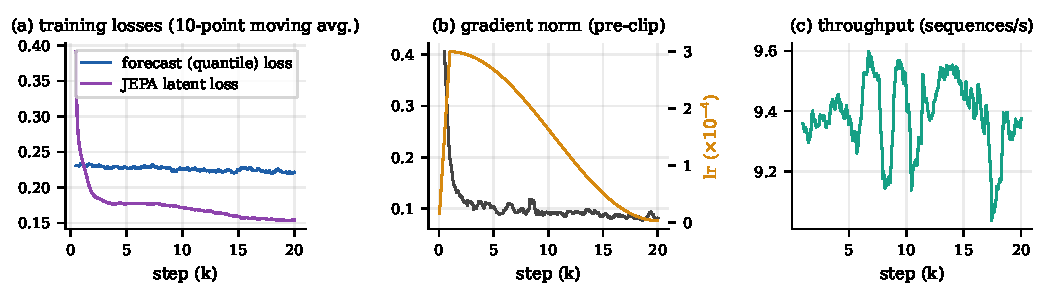
\includegraphics[width=\linewidth]{figs/v3_training.pdf}
\caption{Alma v3 training. (a) forecast and JEPA losses; (b) gradient norm before clipping and learning-rate schedule
(1k warm-up, cosine decay to 1\%); (c) throughput.}
\label{fig:v3train}
\end{figure}

\subsection{Checkpoint selection}
\begin{figure}[H]
\centering
\begin{minipage}{0.48\linewidth}
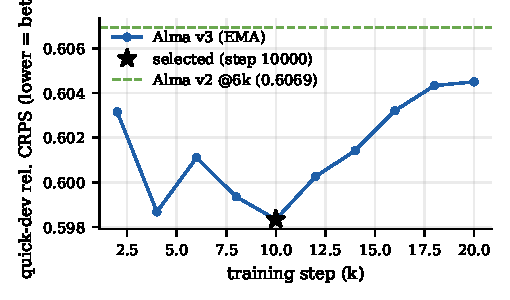
\includegraphics[width=\linewidth]{figs/v3_quickdev.pdf}
\end{minipage}\hfill
\begin{minipage}{0.48\linewidth}
\small
\begin{tabular}{@{}rr@{}}
\toprule
Step & Quick-dev rel.\ CRPS \\
\midrule
2{,}000 & 0.6032 \\
4{,}000 & 0.5987 \\
6{,}000 & 0.6011 \\
8{,}000 & 0.5994 \\
\textbf{10{,}000} & \textbf{0.5983} (selected) \\
12{,}000 & 0.6003 \\
14{,}000 & 0.6014 \\
16{,}000 & 0.6032 \\
18{,}000 & 0.6043 \\
20{,}000 & 0.6045 \\
\midrule
v2 @6k (same routine, 8k ctx) & 0.6069 \\
\bottomrule
\end{tabular}
\end{minipage}
\caption{Quick-dev score of each EMA checkpoint (lower is better). The pre-registered rule selected step 10{,}000.
After step 10k the score rose monotonically while training loss kept falling.}
\label{fig:quickdev}
\end{figure}

The best checkpoint is 1.4\% better than v2 on quick-dev. Most of the gain was reached by step 4k, and the score degraded
steadily over the second half of training, even as training loss fell (Figure~\ref{fig:v3train}a). This is the signature of the
model fitting the training mixture better than it generalises to GIFT-style data.

\subsection{Sealed hold-out test (pre-registered)}
The sealed set contains 8{,}300 GIFT-Eval test windows over 28 tasks (seed 779, up to 300 per task), never used for training,
selection or any earlier grading. Four tasks had no unused windows and were skipped (electricity/W/short, SZ\_TAXI/15T/short,
solar/10T/medium, solar/10T/long), as disclosed in the pre-registration. Inference: v3 at 8{,}192 context with symmetric
averaging; v2 at 2{,}048 (as published); Telos-Small with its own defaults.

\begin{table}[H]
\centering\small
\caption{Sealed test: skill over Seasonal Naive (higher is better).}
\label{tab:sealed_skill}
\begin{tabular}{@{}lcc@{}}
\toprule
Model & CRPS skill & MASE skill \\
\midrule
\textbf{Telos-Small} & \textbf{37.87\%} & \textbf{19.94\%} \\
Alma v3 (ema\_10000) & 35.63\% & 15.65\% \\
Alma v2 (ema\_6000) & 35.56\% & 15.71\% \\
Seasonal Naive & 0.00\% & 0.00\% \\
\bottomrule
\end{tabular}
\end{table}

\begin{table}[H]
\centering\small
\caption{Sealed test: paired comparisons of Alma v3 against each comparator (28 tasks). Ratios below 1 favour v3.
``Beat'' requires $t\ge3$ and passing Holm correction across \{Telos, v2, SN\}.}
\label{tab:sealed_tests}
\setlength{\tabcolsep}{4pt}
\begin{tabular}{@{}l cccc c cccc@{}}
\toprule
 & \multicolumn{5}{c}{CRPS} & \multicolumn{4}{c}{MASE} \\
\cmidrule(lr){2-6}\cmidrule(l){7-10}
v3 vs & gmean ratio & 95\% CI & $t$ & win rate & Beat? & gmean ratio & 95\% CI & $t$ & win rate \\
\midrule
Telos-Small & 1.0362 & [1.0074, 1.0676] & $-2.35$ & 0.29 & \no & 1.0536 & [1.0266, 1.0856] & $-3.68$ & 0.14 \\
Alma v2 & 0.9990 & [0.9788, 1.0187] & 0.10 & 0.61 & \no & 1.0007 & [0.9848, 1.0146] & $-0.10$ & 0.43 \\
Seasonal Naive & 0.6437 & [0.5985, 0.6927] & 12.10 & 1.00 & \yes & 0.8435 & [0.7959, 0.8912] & 5.83 & 0.79 \\
\bottomrule
\end{tabular}
\end{table}

\begin{table}[H]
\centering\small
\caption{Sealed test by forecast length: geometric-mean relative CRPS (lower is better).}
\label{tab:sealed_term}
\begin{tabular}{@{}lccccc@{}}
\toprule
Term & Tasks & Alma v3 & Alma v2 & Telos-Small & v3/Telos (wins) \\
\midrule
Short & 18 & 0.633 & 0.640 & \textbf{0.616} & 1.029 (6) \\
Medium & 5 & 0.635 & 0.620 & \textbf{0.589} & 1.078 (0) \\
Long & 5 & 0.692 & 0.685 & \textbf{0.677} & 1.021 (2) \\
\bottomrule
\end{tabular}
\end{table}

\begin{figure}[H]
\centering
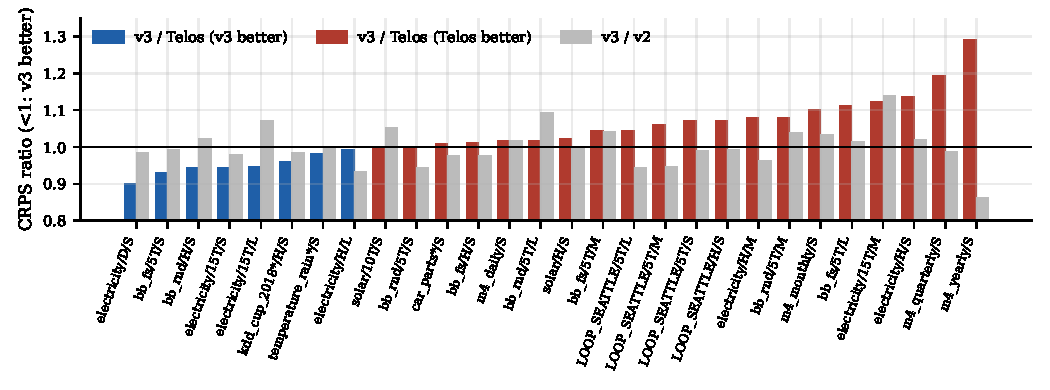
\includegraphics[width=\linewidth]{figs/sealed_per_task.pdf}
\caption{Sealed test, per task, sorted by v3/Telos CRPS ratio. Blue: v3 better than Telos; red: Telos better; grey: v3/v2.
Abbreviations: S/M/L = short/medium/long, bb = bitbrains, fs = fast\_storage, * = with\_missing.}
\label{fig:sealedtask}
\end{figure}

\textbf{Pre-registered outcome.} Telos-Small is better than v3 on the sealed set; the CRPS confidence interval excludes a tie,
and on MASE the difference is significant in Telos's favour ($t=-3.68$). v3 is statistically indistinguishable from v2.
v3 wins on short, high-frequency tasks (electricity/D 0.90, bitbrains\_fast\_storage/5T/short 0.93, electricity/15T/short 0.94)
and on electricity/15T/long (0.95). It loses most on low-frequency M4 series (m4\_yearly 1.29, m4\_quarterly 1.20,
m4\_monthly 1.10) and on medium horizons. Against v2, LOOP\_SEATTLE/5T and electricity/H at medium and long horizons improved by 4--7\%
(0.93--0.96), but other tasks regressed by a similar amount.

\subsection{Full GIFT-Eval benchmark (descriptive, leaderboard)}
v3 was run on all 97 configurations at 8{,}192 context with up to 400 windows per task, as pre-registered (16{,}096\,s on MPS).
The Telos-Small, v1 and v2 runs from earlier in the project used up to 1{,}000 windows. On the 51 tasks with $\le$400 windows in
total, every model saw exactly the same windows; on the remaining 46, v3 was scored on a 400-window subsample. This benchmark
also contains the quick-dev windows used for checkpoint selection, so it is a leaderboard number, not a sealed test.

\begin{table}[H]
\centering\small
\caption{Full GIFT-Eval: skill over Seasonal Naive (higher is better).}
\label{tab:gift}
\begin{tabular}{@{}lc cc cc@{}}
\toprule
 & & \multicolumn{2}{c}{All 97 tasks} & \multicolumn{2}{c}{51 identical-window tasks} \\
\cmidrule(lr){3-4}\cmidrule(l){5-6}
Model & Params & CRPS skill & MASE skill & CRPS skill & MASE skill \\
\midrule
\textbf{Alma v3} @10k & 61.8M & \textbf{39.57} & \textbf{21.93} & \textbf{40.70} & \textbf{23.03} \\
Alma v2 @6k & 27.9M & 38.76 & 20.91 & 39.63 & 22.00 \\
Alma v1 @20k & 21.4M & 38.57 & 21.37 & 39.30 & 22.46 \\
Telos-Small & 50.1M & 38.33 & 19.10 & 37.36 & 16.43 \\
\midrule
v3/Telos CRPS ratio (wins) & & \multicolumn{2}{c}{0.980 (40/97), $t=1.02$} & \multicolumn{2}{c}{0.947 (25/51), $t=1.77$} \\
v3/v2 CRPS ratio & & \multicolumn{2}{c}{0.987} & \multicolumn{2}{c}{0.982} \\
\bottomrule
\end{tabular}
\end{table}

\begin{table}[H]
\centering\small
\caption{Full GIFT-Eval by forecast length (all 97 tasks): geometric-mean relative CRPS and MASE (lower is better).
W = tasks where v3 has lower CRPS than Telos.}
\label{tab:gift_term}
\setlength{\tabcolsep}{3.5pt}
\begin{tabular}{@{}l cccc c cccc@{}}
\toprule
 & \multicolumn{4}{c}{CRPS} & & \multicolumn{4}{c}{MASE} \\
\cmidrule(lr){2-5}\cmidrule(l){7-10}
Term (tasks) & v1 & v2 & v3 & Telos & W & v1 & v2 & v3 & Telos \\
\midrule
Short (55) & \textbf{0.576} & 0.579 & 0.578 & 0.584 & 23 & \textbf{0.755} & 0.758 & 0.759 & 0.773 \\
Medium (21) & 0.639 & 0.642 & \textbf{0.637} & 0.655 & 8 & 0.814 & 0.820 & \textbf{0.797} & 0.849 \\
Long (21) & 0.698 & 0.676 & \textbf{0.646} & 0.669 & 9 & 0.844 & 0.853 & \textbf{0.823} & 0.868 \\
\bottomrule
\end{tabular}
\end{table}

\begin{figure}[H]
\centering
\begin{minipage}{0.49\linewidth}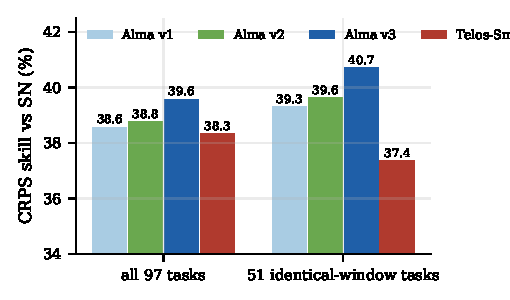
\includegraphics[width=\linewidth]{figs/gift_skill.pdf}\end{minipage}\hfill
\begin{minipage}{0.47\linewidth}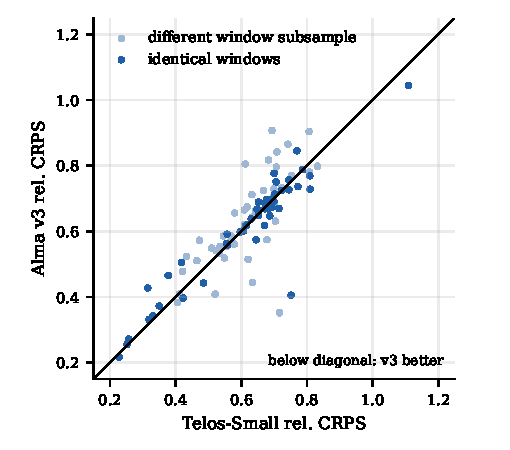
\includegraphics[width=\linewidth]{figs/gift_scatter.pdf}\end{minipage}
\caption{Left: CRPS skill on GIFT-Eval. Right: per-task relative CRPS of v3 vs Telos-Small; dark points were scored on
identical windows.}
\label{fig:gift}
\end{figure}

\textbf{Long horizons.} v3's design goal was the long-horizon gap. On GIFT-Eval it was met: long-term CRPS improved from
0.676 (v2) to \textbf{0.646}, now 3.5\% better than Telos (0.669), and long-term MASE from 0.853 to 0.823. On the sealed set,
however, long-term v3 remained 2.1\% behind Telos (5 tasks).

\textbf{Sensitivity: where the leaderboard advantage comes from.} Table~\ref{tab:dataset} breaks the v3/Telos ratio down by dataset.
Two BizITObs datasets (application and service, 6 tasks) have ratios of 0.50--0.52. \textbf{Excluding those 6 tasks, v3/Telos
on the remaining 91 tasks is 1.023}, i.e.\ Telos is 2.3\% better, which is consistent with the sealed test (1.036). The sealed
set contains no BizITObs task.

\begin{table}[H]
\centering\small
\caption{Full GIFT-Eval, geometric-mean CRPS ratio by dataset (all terms pooled), sorted by v3/Telos.}
\label{tab:dataset}
\begin{tabular}{@{}lrcc@{}}
\toprule
Dataset & Tasks & v3/Telos & v3/v2 \\
\midrule
\DatasetRows
\bottomrule
\end{tabular}
\end{table}

\subsection{Reconciling the two results}
The sealed test and the leaderboard measure different task mixes. The leaderboard spans all 97 configurations, including datasets
where v3 is very strong (BizITObs); the sealed test samples 28 tasks from the pool with unused windows, where low-frequency M4
series and medium horizons weigh more. The sealed test is the stricter instrument: fresh windows, outputs hashed before truth,
and no overlap with the selection sample. \textbf{Our conclusion follows the sealed test: v3 does not beat Telos-Small.}
The defensible public statement is: ``On GIFT-Eval (97 configurations, our harness), Alma v3 scores 39.6\% CRPS skill vs
38.3\% for Telos-Small; on a sealed pre-registered hold-out Telos-Small is 3.6\% better.''

%=====================================================================
\section{Results II --- World models (Alma-WM1 $\rightarrow$ Alma-WM2)}
\subsection{Claim tier and gates}
\begin{table}[H]
\centering\small
\caption{Gate verdicts (validation engine). wm1: no claim tier (Gate 2 failed on one chance overlap in 31 tasks).
wm2: \emph{``The evaluation is leak-free and reproducible''} (Gates 0--3 pass).}
\label{tab:gates}
\setlength{\tabcolsep}{3pt}
\begin{tabular}{@{}l*{15}{c}@{}}
\toprule
Gate & 0 & 1 & 2 & 3 & 4 & 5 & 6 & 7 & 8 & 9 & 10 & 11 & 12 & 13 & 14 \\
\midrule
wm1 & \pass & \pass & \fail & \pass & \fail & \fail & \fail & \fail & \pass & \fail & \fail & \pass & \fail & \pass & \fail \\
wm2 & \pass & \pass & \pass & \pass & \fail & \fail & \fail & \fail & \pass & \fail & \fail & \pass & \fail & \pass & \fail \\
\bottomrule
\end{tabular}
\end{table}

\subsection{Key metrics, wm1 vs wm2}
\begin{table}[H]
\centering\small
\caption{Sealed simulated and real hold-outs. Ratios below 1 favour the world model; $t$ in parentheses.
Threshold column gives the pre-registered pass condition.}
\label{tab:wm}
\setlength{\tabcolsep}{4pt}
\begin{tabular}{@{}llccc@{}}
\toprule
Gate & Check & wm1 & wm2 & Threshold \\
\midrule
4 & One-step (1--16) CRPS vs ARX(24,24) & 1.353 ($-10.7$) & 1.048 ($-2.8$) & $t\ge3$ \\
5.1 & Rollout vs ARX, 17--64 / 65--256 / 257--512 & 1.18 / 1.18 / 1.26 & \textbf{0.92 / 0.87 / 0.93} & $t\ge3$ each \\
5.1 & Error growth CRPS(257--512)/CRPS(1--16) & 2.07 & 1.83 & $\le10$ \pass \\
5.6 & Constraint violations (median $<0$) & 15.4\% & 19.1\% & $\le1\%$ (mis-specified, A3) \\
6.1 & Action-aware vs action-blind & 0.751 (15.1) & \textbf{0.634 (20.4)} & $t\ge3$ \pass \\
6.2 & Effect-sign accuracy (ARX) & 0.954 (0.925) & \textbf{0.971} (0.922) & $\ge0.90$ \pass \\
6.2 & Monotone dose sweeps & 0.923 & \textbf{0.954} & $\ge0.95$ \pass \\
6.5* & Counterfactual CRPS vs ARX & 1.427 ($-8.8$) & 0.981 (0.7) & $t\ge3$ \\
7 & Coverage of 80\% / 60\% intervals & 75.3\% / 55.4\% & 76.9\% / 57.1\% & $\pm2$\,pp \\
7.3 & Conformal 80\% coverage & 79.9\% & 79.6\% & $\pm2$\,pp \pass \\
7.4 & OOD AUROC, Mahalanobis (disagreement) & 0.532 (0.584) & 0.525 (0.688) & $\ge0.75$ \\
8.10 & Placebo: true vs shuffled actions & 0.637 (20.5) & 0.530 (26.5) & $t\ge3$ \pass \\
8.10 & Placebo: random actions vs blind & 1.162 & 1.359 & must not beat \pass \\
8.10 & Placebo: 16-step time-shifted actions & 0.677 (18.2) & 0.645 (20.2) & $t\ge3$ \pass \\
9.7 & Held-out family (tanks): aware/ARX & 1.402 & \textbf{0.919} & descriptive \\
10.1 & Latent effective rank & 146.3 & 177.6 & $\ge16$ \pass \\
12 & MPC real cost vs default plan & 0.652 (3.3) & \textbf{0.418 (7.9)} & $t\ge3$ \\
12 & MPC real cost vs ARX-MPC & 1.691 ($-5.0$) & 1.087 ($-1.4$) & $t\ge3$ \\
12.1 & Imagined vs real gain & 1.131 & 1.078 & $\ge0.70$ \pass \\
4.2 & REAL: vs Seasonal Naive & 0.645 (7.3) & 0.638 (11.1) & $t\ge3$ \\
4.2 & REAL: vs Telos-Small (wins) & 1.038 (0.41) & 1.037 (0.24) & $t\ge3$ \\
4.2 & REAL: non-inferiority vs v2 (CI upper) & 1.014 (1.026) & 1.000 (1.000) & $\le1.01$ \\
\bottomrule
\end{tabular}
\end{table}

\begin{figure}[H]
\centering
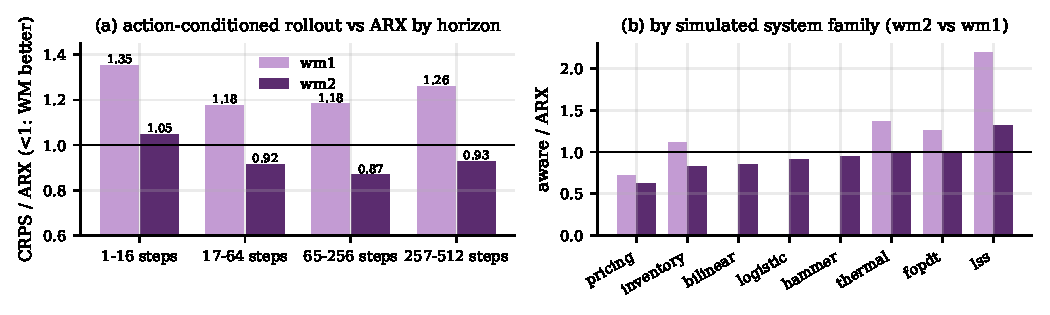
\includegraphics[width=\linewidth]{figs/wm_horizon_family.pdf}
\caption{(a) Action-conditioned rollout CRPS relative to ARX(24,24) by horizon bucket. (b) By simulated system family;
wm1 had 5 families, wm2 has 8.}
\label{fig:wmh}
\end{figure}

\begin{figure}[H]
\centering
\begin{minipage}{0.49\linewidth}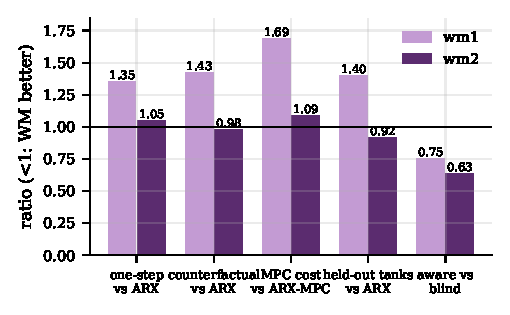
\includegraphics[width=\linewidth]{figs/wm_key_ratios.pdf}\end{minipage}\hfill
\begin{minipage}{0.49\linewidth}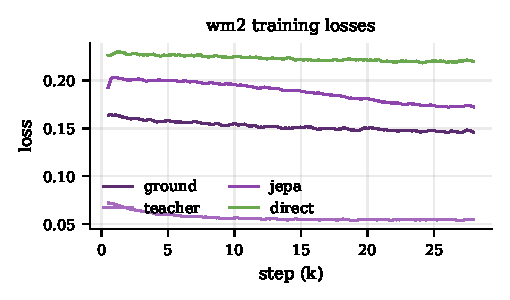
\includegraphics[width=\linewidth]{figs/wm2_training.pdf}\end{minipage}
\caption{Left: key world-model ratios, wm1 vs wm2 (below 1 = world model better). Right: wm2 training losses
(28k steps, 18.3 sequences/s).}
\label{fig:wmkey}
\end{figure}

\subsection{Interpretation}
\begin{itemize}
\item \textbf{What wm2 does well.} It beats ARX at every horizon beyond 16 steps; it transfers to the never-seen tanks family
(0.919); it beats ARX in 6 of 8 families (pricing 0.63, inventory 0.82, bilinear 0.86, logistic 0.92, hammer 0.95, thermal 0.98);
all placebo tests pass with larger margins than wm1; and its plans reduce real cost by 58\% vs the default plan ($t=7.9$).
\item \textbf{Where it fails.} One-step accuracy (1.048) and linear state-space systems (lss 1.32), where ARX is the correct model
class; counterfactual accuracy is better than ARX on average but not significantly (0.981, $t=0.7$); MPC ties ARX-MPC (1.087,
$t=-1.4$).
\item \textbf{Calibration and OOD.} Raw 80\% intervals cover 76.9\%; a conformal layer fixes this (79.6\%). The Mahalanobis OOD flag
does not track error (0.525); the disagreement score improved to 0.69 but is below 0.75.
\item \textbf{Probes.} Linear decodability of system parameters improved (thermal.a $R^2$ 0.27$\to$0.66, fopdt.$\tau$ 0.03$\to$0.23,
inventory.lag $-0.05\to0.17$), but fopdt.delay is still not decodable ($R^2=-0.04$), so gate 10.1 fails.
\item \textbf{Real data.} wm2's forecasting path is the frozen v2, so its real-data results equal v2's by construction.
\end{itemize}

%=====================================================================
\section{Engineering incidents and pre-registration amendments}
\label{sec:incidents}
\begin{itemize}
\item \textbf{v3 MPS out-of-memory (3 attempts, no checkpoints).} A batch of 32 at 8k context exceeded 16\,GB unified memory.
Fix: gradient accumulation in chunks of 8 (\code{--micro-bs 8}); the effective batch stays 32; peak memory $\approx$7\,GB.
\item \textbf{v3 infinite gradient norm on 8k batches.} Zero-initialising the coarse embedding put coarse tokens at RMSNorm's
$x=0$ singularity, producing gradients $\sim10^{27}$. Fix: initialise it as the grown fine embedding applied to pair-averaged
patches. After the fix the 8k-batch gradient norm was 0.10 and the loss on that batch dropped from 0.327 to 0.240; exactness at
$\le$4k was unchanged ($8.6\times10^{-6}$). Both fixes were recorded as Amendment V3-A1 \emph{before any training step} and
before any sealed output; v3 restarted from step 0.
\item \textbf{wm2 Gate 5.6 mis-specified (Amendment A3).} On the DEBUG harness the ground truth itself has negative medians in
4.9\% (inventory) and 20.3\% (pricing) of cases, so a $\le$1\% threshold cannot be met by a correct model. 5.6 is still computed and
counted as not passed.
\item \textbf{wm1 Gate 2.2.} One chance exact-match overlap in 31 tasks; wm2 added an entropy floor and a label scan (Amendment A2),
and found 0 hits.
\item \textbf{Throughput.} Other applications caused swap pressure (wm2 fell from 18.5 to 12.4 sequences/s until they were closed).
A pause/resume mechanism (SIGSTOP/SIGCONT) was used once without loss of progress.
\end{itemize}

%=====================================================================
\section{Claims we can and cannot make}
\begin{table}[H]
\centering\small
\caption{Claim audit.}
\label{tab:claims}
\begin{tabular}{@{}p{0.62\linewidth}p{0.08\linewidth}p{0.24\linewidth}@{}}
\toprule
Claim & OK? & Evidence \\
\midrule
v3 scores higher CRPS and MASE skill than Telos-Small on full GIFT-Eval (our harness) & \yes & Table~\ref{tab:gift} \\
v3 closes the long-horizon gap on GIFT-Eval (0.646 vs Telos 0.669) & \yes & Table~\ref{tab:gift_term} \\
v3 beats Seasonal Naive on the sealed set (Holm, $t=12.1$) & \yes & Table~\ref{tab:sealed_tests} \\
v3 significantly beats Telos-Small & \no & sealed 1.036, $t=-2.35$ \\
v3 improves on v2 on fresh data & \no & sealed 0.999, $t=0.10$ \\
Alma-WM2's evaluation is leak-free and reproducible & \yes & Gates 0--3 \\
Alma-WM2 beats ARX on long-horizon action-conditioned rollouts and on a held-out family & \yes\,(desc.) & Table~\ref{tab:wm} \\
Alma-WM2 is a validated world model (counterfactuals / planning beat baselines) & \no & 6.5*, 12 \\
Alma-WM2 is calibrated and detects OOD inputs & \no & 7, 7.4 \\
Any causal claim about real systems & \no & no real interventional data \\
\bottomrule
\end{tabular}
\end{table}

%=====================================================================
\section{Threats to validity}
\begin{itemize}
\item \textbf{Not independent.} All models were built and validated by the same agent (stated in the model cards).
\item \textbf{One training seed} per model; seed variance is unmeasured (gate 10.4 fails for this reason).
\item \textbf{Window caps differ} on the GIFT leaderboard (400 for v3, 1{,}000 for the others) on 46 of 97 tasks;
the identical-window subset (51 tasks) is reported separately.
\item \textbf{Telos-Small is run on our harness}, where it scores 38.33\%, below its model card's 43.21\% (different quantile set
and window cap). Every model is affected identically.
\item \textbf{Selection overlap.} The leaderboard includes the quick-dev windows used to pick v3's checkpoint; the sealed set does not.
\item \textbf{Small sealed sample.} 28 tasks; 4 further tasks could not be sampled.
\item \textbf{Simulated world-model evidence.} All action and planning results are on simulators; real interventional data is absent.
\end{itemize}

%=====================================================================
\section{Compute}
\begin{table}[H]
\centering\small
\caption{Compute on one Apple M4 (16\,GB unified memory, MPS).}
\begin{tabular}{@{}lll@{}}
\toprule
Run & Wall-clock & Notes \\
\midrule
Alma v1 & 7.0\,h & 20k steps $\times$ 64 \\
Alma v2 & 3.5\,h & 10k steps $\times$ 32 \\
Alma-WM2 & $\approx$13.6\,h of training & 28k steps $\times$ 32 at 18.3 seq/s (excluding pauses) \\
Alma v3 & 19.3\,h & 20k steps $\times$ 32 at 9.39 seq/s, incl.\ 10 quick-dev evaluations \\
v3 sealed prediction (4 models, 8{,}300 windows) & 11\,min & Telos on CPU \\
v3 full GIFT-Eval & 4.5\,h & 97 configs, 8k context \\
\bottomrule
\end{tabular}
\end{table}

%=====================================================================
\section{Conclusions and next steps}
\textbf{Conclusions.}
\begin{enumerate}
\item All six v3 plan items were implemented and executed; the 12$\times$512 growth was exact and training was stable.
\item v3 leads Telos-Small on the public GIFT-Eval aggregate (39.57\% vs 38.33\% CRPS skill), largely through BizITObs and
long horizons, but \textbf{does not beat it on the sealed pre-registered test} (Telos 3.6\% better).
\item Model size is not the bottleneck: $2.2\times$ more parameters and $2\times$ more steps left the sealed score unchanged
relative to v2, and quick-dev degraded after 10k steps.
\item Alma-WM2 is a genuine improvement over wm1 on every major axis and earns the first claim tier, but does not yet
satisfy the gates that would make it a validated world model.
\end{enumerate}

\textbf{Next steps.}
\begin{enumerate}
\item \textbf{v4: data, not size.} Substantially larger and more diverse real pretraining data, prioritising low-frequency series
(yearly/quarterly/monthly), medium horizons and the remaining GiftEvalPretrain shards, with a leakage scan; shorter runs per data
refresh; checkpoint averaging (registered before sealing).
\item \textbf{wm3.} v3 as the frozen forecasting path; a conformal layer shipped in the model; a $k$-NN or per-family OOD head;
a per-horizon ARX prior gate; a corrected gate 5.6; several training seeds; and a source of real interventional data.
\item \textbf{Fully matched leaderboard.} Re-run v3 at 1{,}000 windows per task.
\end{enumerate}

%=====================================================================
\appendix
\section{Sealed test, per task}
\begin{table}[H]
\centering\small
\caption{Sealed test (seed 779), relative CRPS vs Seasonal Naive per task (lower is better; best in bold) and ratios.}
\label{tab:sealed_pertask}
\begin{tabular}{@{}lccccc@{}}
\toprule
Task & Alma v3 & Alma v2 & Telos-Small & v3/Telos & v3/v2 \\
\midrule
\SealedRows
\bottomrule
\end{tabular}
\end{table}

\section{Reproducibility}
\begin{itemize}
\item Selected v3 checkpoint: \code{runs/alma\_v3/ema\_10000.pt}; v3 validation run \code{validation\_runs/AlmaV3\_fc\_20261116T2349Z}
(pre-registration, amendment V3-A1, \code{manifest.json} with seal and truth-load times).
\item wm2 validation run \code{validation\_runs/AlmaWM2\_wm2\_20261116T2254Z}, manifest sha256 \code{09e63745cfafc78e\ldots};
rerun with \code{make validate RUN=AlmaWM2\_wm2\_20261116T2254Z}.
\item GIFT-Eval results: \code{results/alma\_v3\_gift.json}, \code{results/telos\_gift.json}, \code{results/alma\_v2\_6000\_gift.json}.
\item Every number and figure in this report is regenerated from those files by \code{report/final/make\_figs.py} and
\code{report/final/make\_tables.py} (output \code{numbers.json}).
\end{itemize}

\end{document}
